\documentclass[12pt,letterpaper]{article}
\usepackage{graphicx,textcomp}
\usepackage{natbib}
\usepackage{setspace}
\usepackage{fullpage}
\usepackage{color}
\usepackage[reqno]{amsmath}
\usepackage{amsthm}
\usepackage{fancyvrb}
\usepackage{amssymb,enumerate}
\usepackage[all]{xy}
\usepackage{endnotes}
\usepackage{lscape}
\newtheorem{com}{Comment}
\usepackage{float}
\usepackage{hyperref}
\newtheorem{lem} {Lemma}
\newtheorem{prop}{Proposition}
\newtheorem{thm}{Theorem}
\newtheorem{defn}{Definition}
\newtheorem{cor}{Corollary}
\newtheorem{obs}{Observation}
\usepackage[compact]{titlesec}
\usepackage{dcolumn}
\usepackage{tikz}
\usetikzlibrary{arrows}
\usepackage{multirow}
\usepackage{xcolor}
\newcolumntype{.}{D{.}{.}{-1}}
\newcolumntype{d}[1]{D{.}{.}{#1}}
\definecolor{light-gray}{gray}{0.65}
\usepackage{url}
\usepackage{listings}
\usepackage{color}
\usepackage{ dsfont }

\definecolor{codegreen}{rgb}{0,0.6,0}
\definecolor{codegray}{rgb}{0.5,0.5,0.5}
\definecolor{codepurple}{rgb}{0.58,0,0.82}
\definecolor{backcolour}{rgb}{0.95,0.95,0.92}

\lstdefinestyle{mystyle}{
	backgroundcolor=\color{backcolour},   
	commentstyle=\color{codegreen},
	keywordstyle=\color{magenta},
	numberstyle=\tiny\color{codegray},
	stringstyle=\color{codepurple},
	basicstyle=\footnotesize,
	breakatwhitespace=false,         
	breaklines=true,                 
	captionpos=b,                    
	keepspaces=true,                 
	numbers=left,                    
	numbersep=5pt,                  
	showspaces=false,                
	showstringspaces=false,
	showtabs=false,                  
	tabsize=2
}
\lstset{style=mystyle}
\newcommand{\Sref}[1]{Section~\ref{#1}}
\newtheorem{hyp}{Hypothesis}

\title{Problem Set 3}
\date{Due: November 11, 2024}
\author{Applied Stats/Quant Methods 1}


\begin{document}
	\maketitle
	\section*{Instructions}
	\begin{itemize}
		\item Please show your work! You may lose points by simply writing in the answer. If the problem requires you to execute commands in \texttt{R}, please include the code you used to get your answers. Please also include the \texttt{.R} file that contains your code. If you are not sure if work needs to be shown for a particular problem, please ask.
	\item Your homework should be submitted electronically on GitHub.
	\item This problem set is due before 23:59 on Sunday November 11, 2024. No late assignments will be accepted.

	\end{itemize}

		\vspace{.25cm}
	
\noindent In this problem set, you will run several regressions and create an add variable plot (see the lecture slides) in \texttt{R} using the \texttt{incumbents\_subset.csv} dataset. Include all of your code.

	\vspace{.5cm}
\section*{Question 1}
\vspace{.25cm}

Dataset is imported with:
\lstinputlisting[language=R, firstline=11, lastline=11]{PS03_victor_gomez_24362159.R}  

\noindent We are interested in knowing how the difference in campaign spending between incumbent and challenger affects the incumbent's vote share. 
	\begin{enumerate}
		\item Run a regression where the outcome variable is \texttt{voteshare} and the explanatory variable is \texttt{difflog}.	 \\
			The linear regression is done by the folowing code:
			\lstinputlisting[language=R, firstline=21, lastline=21]{PS03_victor_gomez_24362159.R}  
			which gives:
			\begin{verbatim}
				> lm1
				Call:
				lm(formula = voteshare ~ difflog, data = df)
				
				Coefficients:
				(Intercept)      difflog  
				    0.57903      0.04167 
			\end{verbatim}	
		\item Make a scatterplot of the two variables and add the regression line. 
			The scatter plot is made by the folowing code:
			\lstinputlisting[language=R, firstline=24, lastline=29]{PS03_victor_gomez_24362159.R}  
			Which gives the Fig.\ref{fig:lm_1}. \\
				
			\begin{figure}[h!]\centering
				\caption{\footnotesize Regression between voteshare and difflog}
				\label{fig:lm_1}
				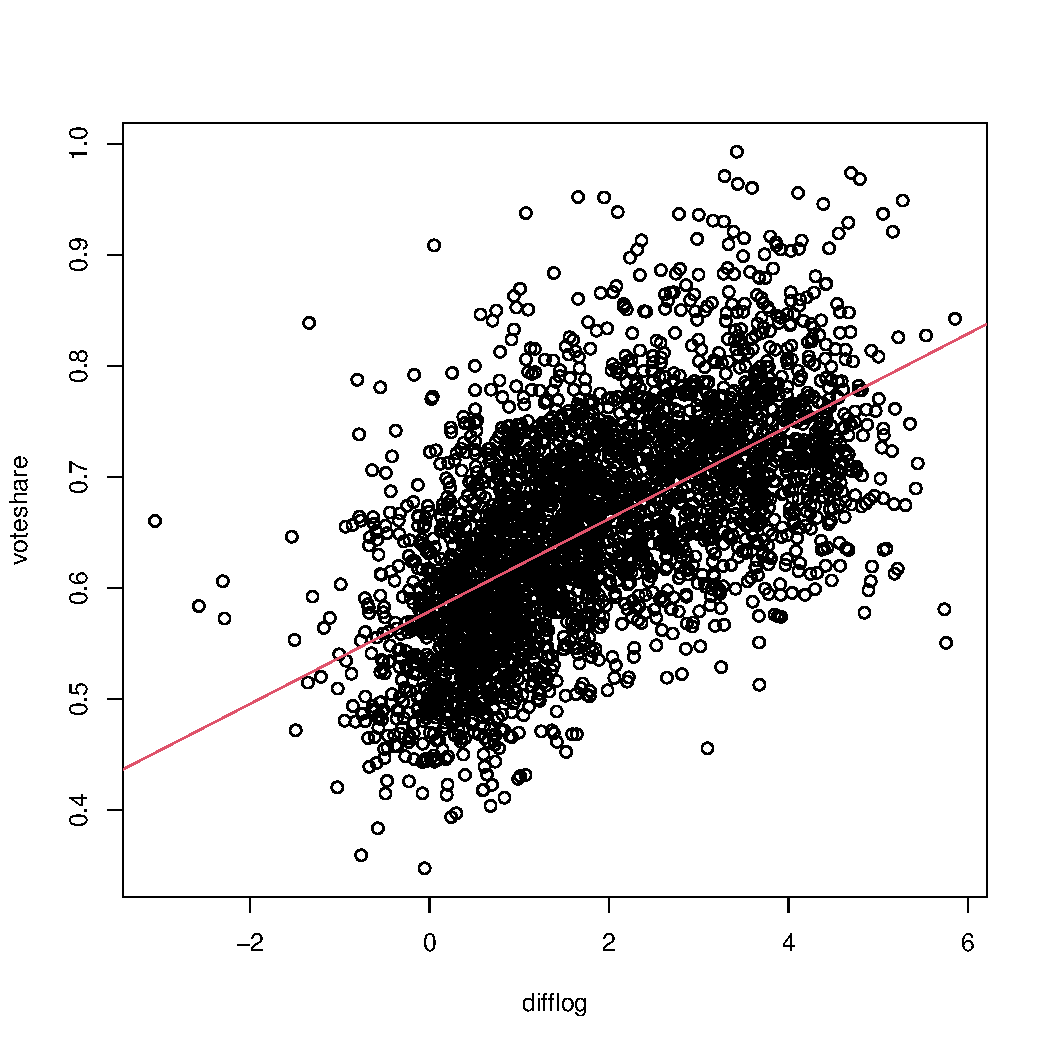
\includegraphics[width=.85\textwidth]{lm1.pdf}
			\end{figure}
		\item Save the residuals of the model in a separate object.\\
			It is done as folows.\\
			
			\lstinputlisting[language=R, firstline=31, lastline=31]{PS03_victor_gomez_24362159.R}  
			
			and plot with:\\
			\lstinputlisting[language=R, firstline=32, lastline=36]{PS03_victor_gomez_24362159.R}  

			\begin{figure}[h!]\centering
				\caption{\footnotesize Residuals of the linear regression between voteshare and difflog}
				\label{fig:res_1}
				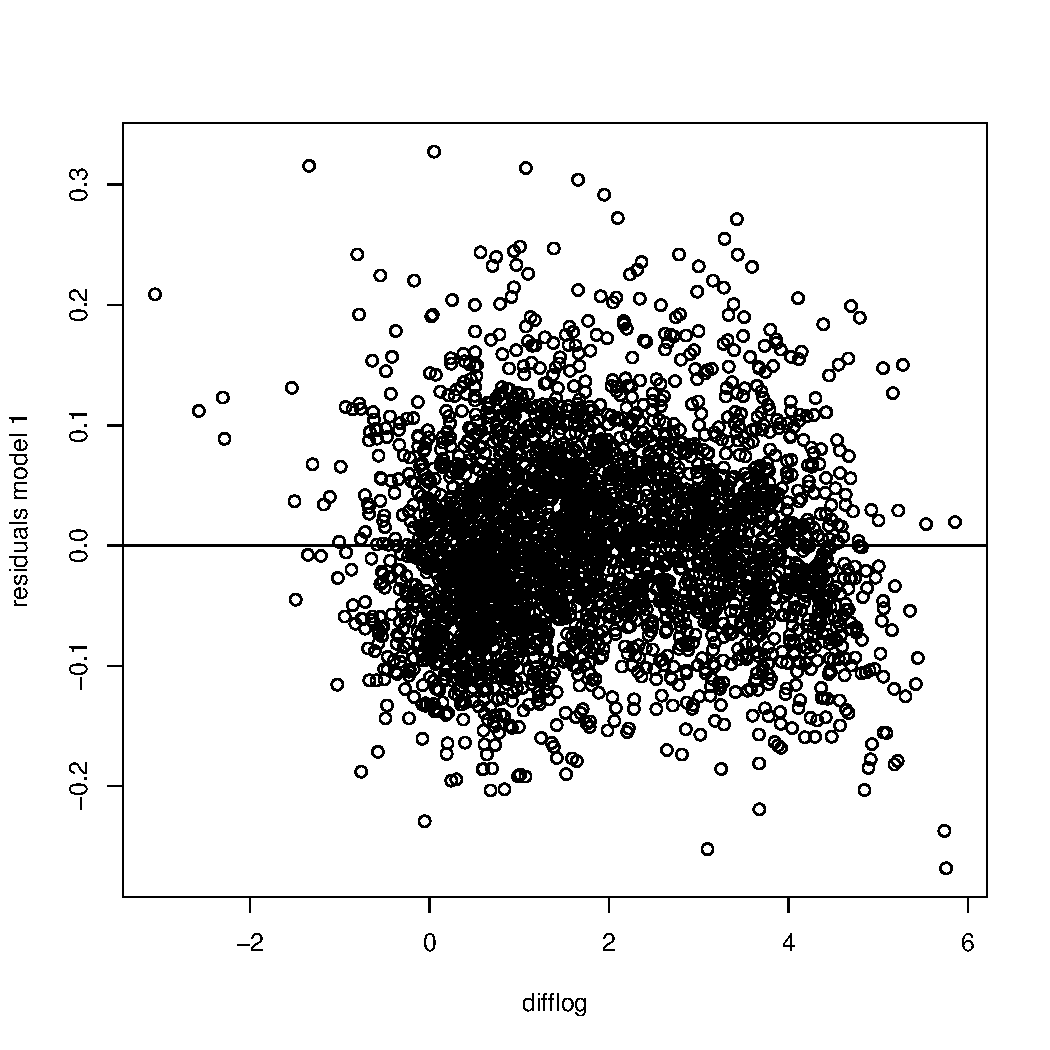
\includegraphics[width=.85\textwidth]{res1.pdf}
			\end{figure}			
			Fig. \ref{fig:res_1} shows residuals are randomly arranged around 0, which means that the linear regression is accurate here.

		\item Write the prediction equation.\\
			Considering $\hat{Y}$ the predictor of \texttt{voteshare}, \\ $\hat{\beta_1}$ the calculated coefficient,\\ $\hat{\beta_0}$ the calculated intercept,\\ $X$ the
			 \texttt{difflog} \\ and the margin of error $\epsilon \leadsto  \mathcal{N} ( \mu, \sigma ), ( \mu, \sigma ) \in \mathds{R}\times \mathds{R}^+$, \\
			 the linear regression model gives:
			
			\begin{align*}
				 \hat{Y} &= \hat{\beta_1} X + \hat{\beta_0} + \epsilon \\
				&=  0.04167 X + 0.57903 + \epsilon
			\end{align*}
	\end{enumerate}
	
\newpage

\section*{Question 2}
\noindent We are interested in knowing how the difference between incumbent and challenger's spending and the vote share of the presidential candidate of the incumbent's party are related.	\vspace{.25cm}
	\begin{enumerate}
		\item Run a regression where the outcome variable is \texttt{presvote} and the explanatory variable is \texttt{difflog}. \\
			The linear regression is done by the folowing code:
			\lstinputlisting[language=R, firstline=45, lastline=45]{PS03_victor_gomez_24362159.R}  
			which gives:
			\begin{verbatim}
				> lm2
				Call:
				lm(formula = presvote ~ difflog, data = df)
				
				Coefficients:
				(Intercept)      difflog  
				    0.50758      0.02384 
			\end{verbatim}

		\item Make a scatterplot of the two variables and add the regression line. \\
			The scatter plot is made by the folowing code:
			\lstinputlisting[language=R, firstline=48, lastline=52]{PS03_victor_gomez_24362159.R}  
			Which gives the Fig.\ref{fig:lm_2}. \\
				
			\begin{figure}[h!]\centering
				\caption{\footnotesize Regression between presvote and difflog}
				\label{fig:lm_2}
				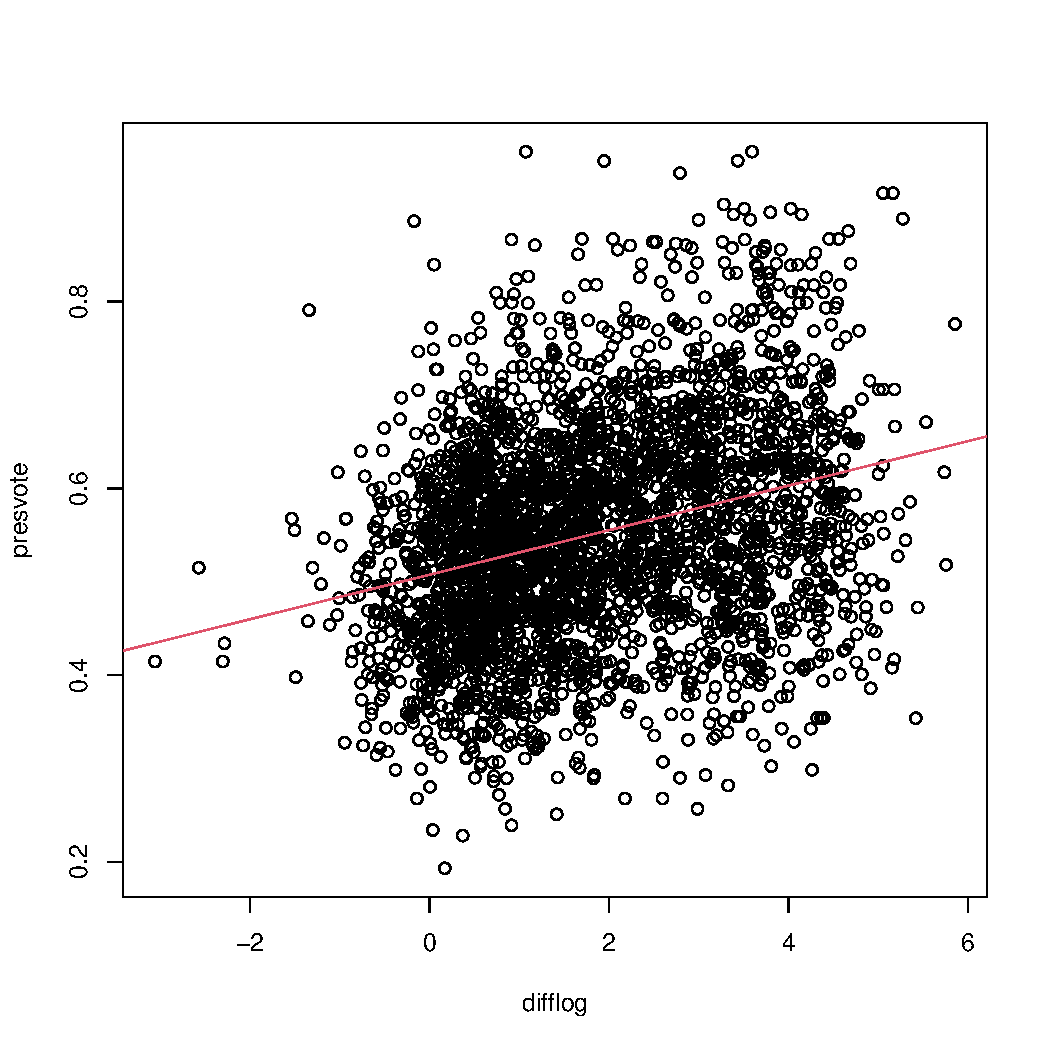
\includegraphics[width=.85\textwidth]{lm2.pdf}
			\end{figure}
		\item Save the residuals of the model in a separate object.\\
			It is done as folows.\\
			
			\lstinputlisting[language=R, firstline=55, lastline=55]{PS03_victor_gomez_24362159.R}  
			
			and plot with:\\
			\lstinputlisting[language=R, firstline=56, lastline=60]{PS03_victor_gomez_24362159.R}  

			\begin{figure}[h!]\centering
				\caption{\footnotesize Residuals of the linear regression between presvote and difflog}
				\label{fig:res_2}
				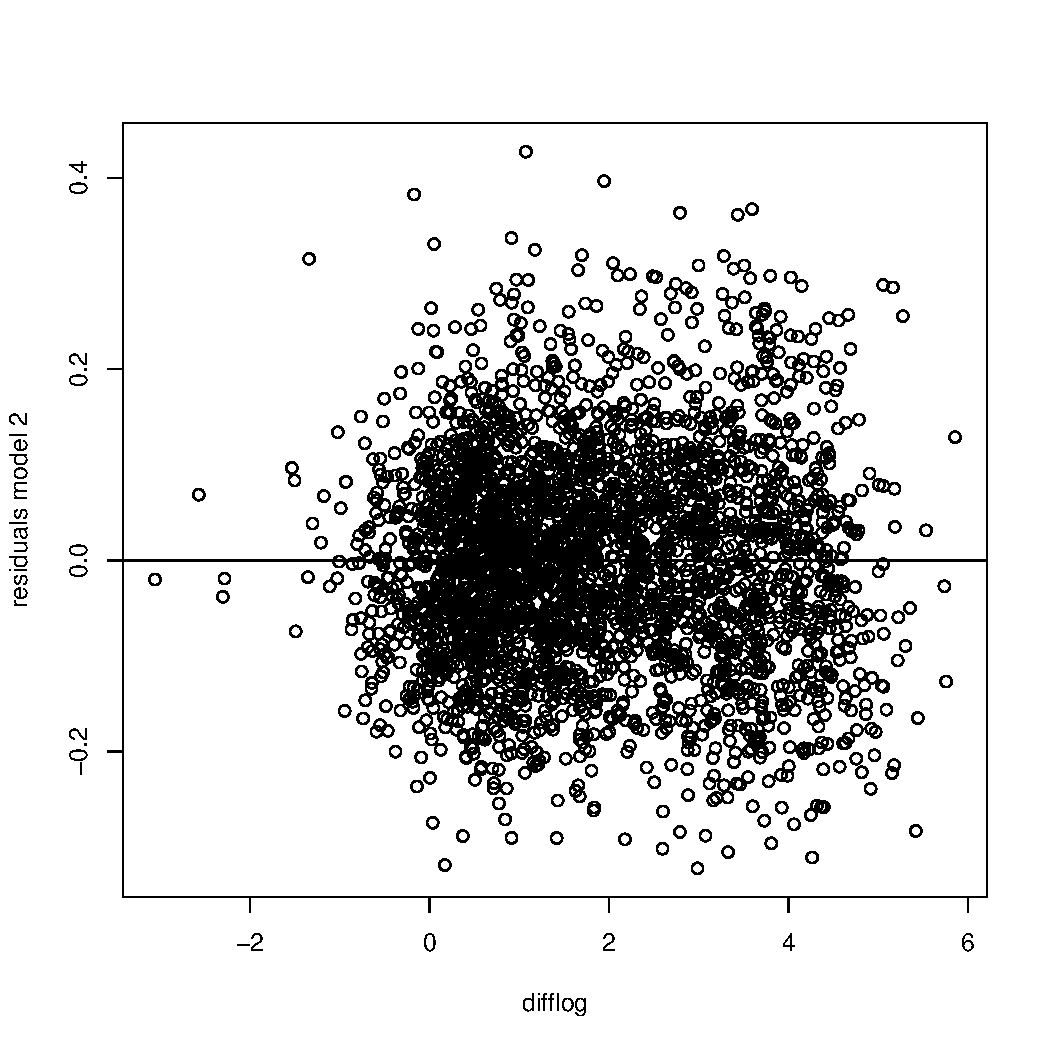
\includegraphics[width=.85\textwidth]{res2.pdf}
			\end{figure}			
			Fig. \ref{fig:res_2} shows residuals are randomly arranged around 0, which means that the linear regression is accurate here.			

		\item Write the prediction equation.
			Considering $\hat{Y}$ the predictor of \texttt{presvote}, \\ $\hat{\beta_1}$ the calculated coefficient,\\ $\hat{\beta_0}$ the calculated intercept,\\ $X$ the
			 \texttt{difflog} \\ and the margin of error $\epsilon \leadsto  \mathcal{N} ( \mu, \sigma ), ( \mu, \sigma ) \in \mathds{R}\times \mathds{R}^+$, \\
			 the linear regression model gives:
			
			\begin{align*}
				 \hat{Y} &= \hat{\beta_1} X + \hat{\beta_0} + \epsilon \\
				&=   0.02384 X +  0.50758   + \epsilon
			\end{align*}
	\end{enumerate}
	
	\newpage	
\section*{Question 3}

\noindent We are interested in knowing how the vote share of the presidential candidate of the incumbent's party is associated with the incumbent's electoral success.
	\vspace{.25cm}
	\begin{enumerate}
		\item Run a regression where the outcome variable is \texttt{voteshare} and the explanatory variable is \texttt{presvote}.\\
			The linear regression is done by the folowing code:
			\lstinputlisting[language=R, firstline=69, lastline=69]{PS03_victor_gomez_24362159.R}  
			which gives:
			\begin{verbatim}
				> lm3

				Call:
				lm(formula = voteshare ~ presvote, data = df)
				
				Coefficients:
				(Intercept)     presvote  
				     0.4413       0.3880  
			\end{verbatim}	
		\item Make a scatterplot of the two variables and add the regression line. \\
			The scatter plot is made by the folowing code:
			\lstinputlisting[language=R, firstline=72, lastline=76]{PS03_victor_gomez_24362159.R}  
			Which gives the Fig.\ref{fig:lm_3}. \\
				
			\begin{figure}[h!]\centering
				\caption{\footnotesize Regression between voteshare and presvote}
				\label{fig:lm_3}
				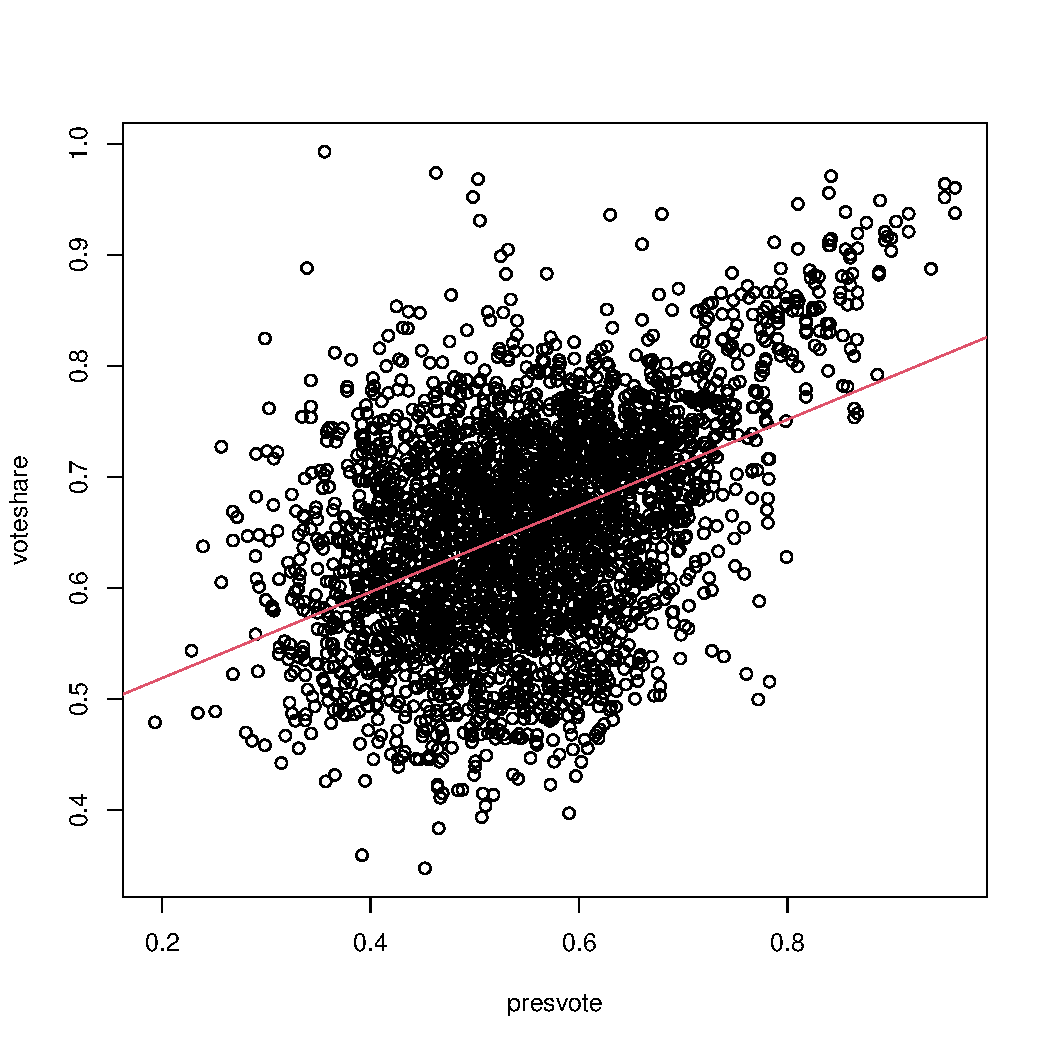
\includegraphics[width=.85\textwidth]{lm3.pdf}
			\end{figure}
			The residuals of the model are given by:\\
			
			\lstinputlisting[language=R, firstline=79, lastline=79]{PS03_victor_gomez_24362159.R}  
			
			and plotted with:\\
			\lstinputlisting[language=R, firstline=80, lastline=84]{PS03_victor_gomez_24362159.R}  

			\begin{figure}[h!]\centering
				\caption{\footnotesize Residuals of the linear regression between voteshare and presvote}
				\label{fig:res_3}
				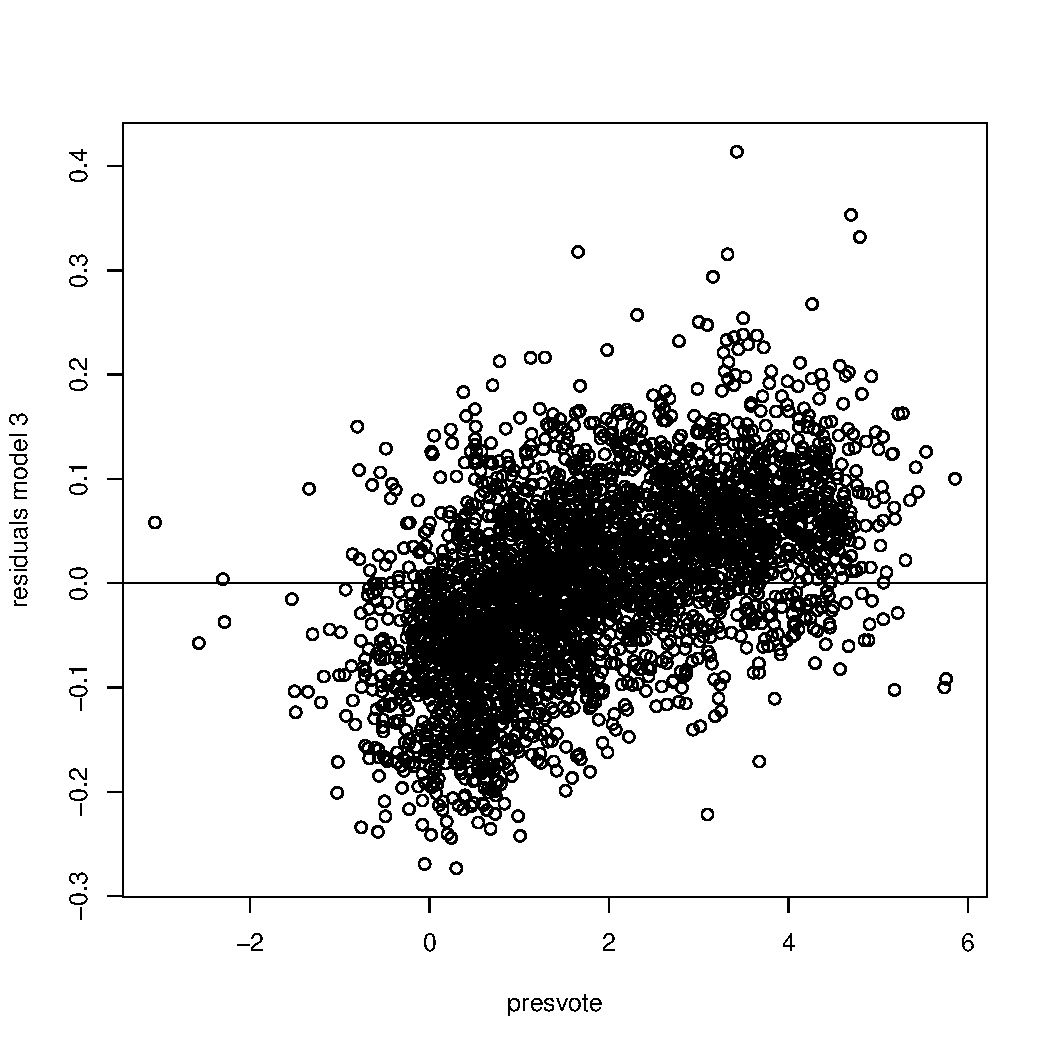
\includegraphics[width=.85\textwidth]{res3.pdf}
			\end{figure}			
			Fig. \ref{fig:res_3} shows residuals are not  randomly arranged around 0, which means that the linear regression is not accurate here. A squared or logarithmic relation are prehaps to expect.
		\item Write the prediction equation.
			Considering $\hat{Y}$ the predictor of \texttt{voteshare}, \\ $\hat{\beta_1}$ the calculated coefficient,\\ $\hat{\beta_0}$ the calculated intercept,\\ $X$ the
			 \texttt{presvote} \\ and the margin of error $\epsilon \leadsto  \mathcal{N} ( \mu, \sigma ), ( \mu, \sigma ) \in \mathds{R}\times \mathds{R}^+$, \\
			 the linear regression model gives:
			
			\begin{align*}
				 \hat{Y} &= \hat{\beta_1} X + \hat{\beta_0} + \epsilon \\
				&=   0.3880  X +  0.4413  + \epsilon
			\end{align*}
	\end{enumerate}
	

\newpage	
\section*{Question 4}
\noindent The residuals from part (a) tell us how much of the variation in \texttt{voteshare} is $not$ explained by the difference in spending between incumbent and challenger. The residuals in part (b) tell us how much of the variation in \texttt{presvote} is $not$ explained by the difference in spending between incumbent and challenger in the district.
	\begin{enumerate}
		\item Run a regression where the outcome variable is the residuals from Question 1 and the explanatory variable is the residuals from Question 2.	\\
			The linear regression is done by the folowing code:
			\lstinputlisting[language=R, firstline=93, lastline=93]{PS03_victor_gomez_24362159.R}  
			which gives:
			\begin{verbatim}
				> lm4

				Call:
				lm(formula = lm1_residuals ~ lm2_residuals, data = df)
				
				Coefficients:
				  (Intercept)  lm2_residuals  
				   -5.934e-18      2.569e-01  
			\end{verbatim}	

		\item Make a scatterplot of the two residuals and add the regression line. 	\\
			The scatter plot is made by the folowing code:
			\lstinputlisting[language=R, firstline=96, lastline=100]{PS03_victor_gomez_24362159.R}  
			Which gives the Fig.\ref{fig:lm_4}. \\
				
			\begin{figure}[h!]\centering
				\caption{\footnotesize Regression between residuals of two first models}
				\label{fig:lm_4}
				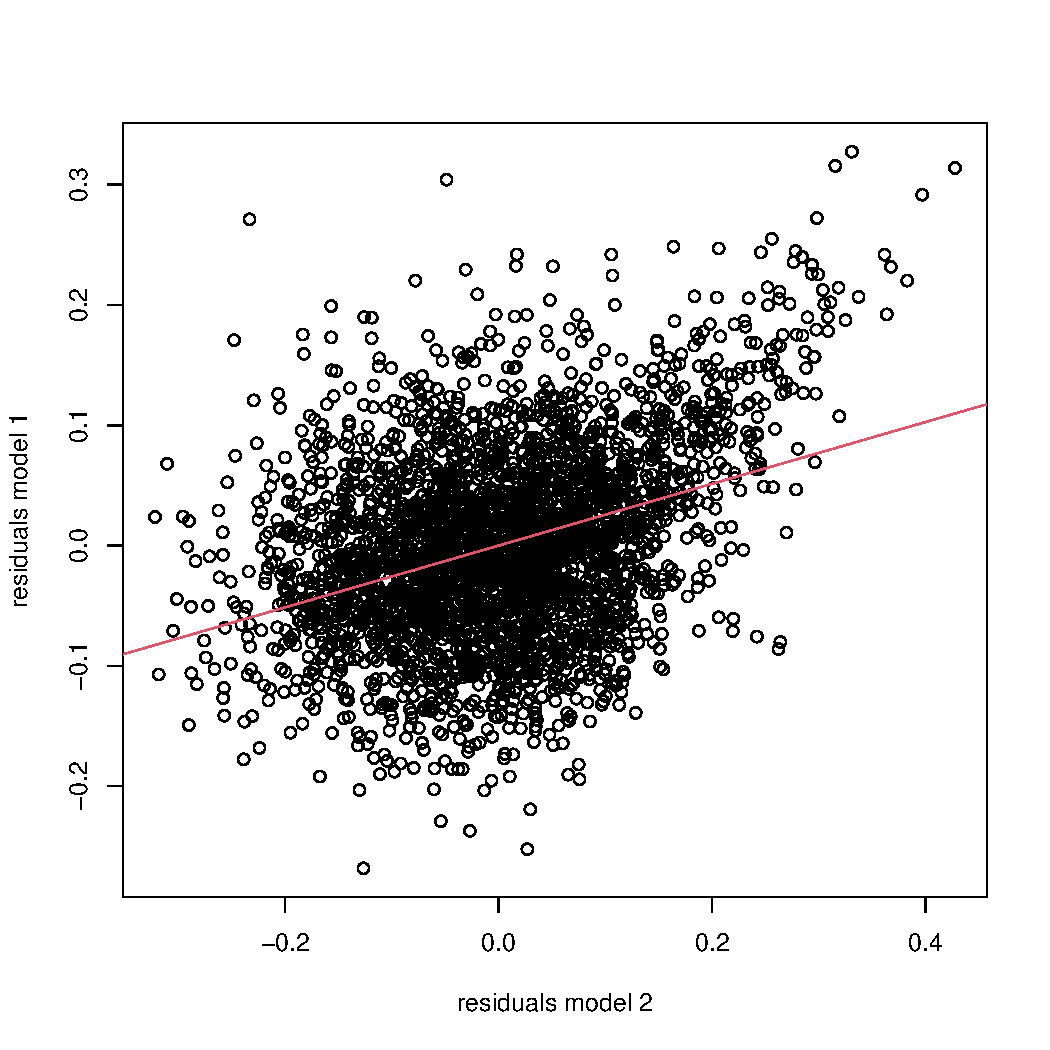
\includegraphics[width=.85\textwidth]{lm4.pdf}
			\end{figure}
			The residuals of the model are given by:\\
			
			\lstinputlisting[language=R, firstline=103, lastline=103]{PS03_victor_gomez_24362159.R}  
			
			and plotted with:\\
			\lstinputlisting[language=R, firstline=104, lastline=108]{PS03_victor_gomez_24362159.R}  

			\begin{figure}[h!]\centering
				\caption{\footnotesize Residuals of the linear regression between voteshare and presvote}
				\label{fig:res_4}
				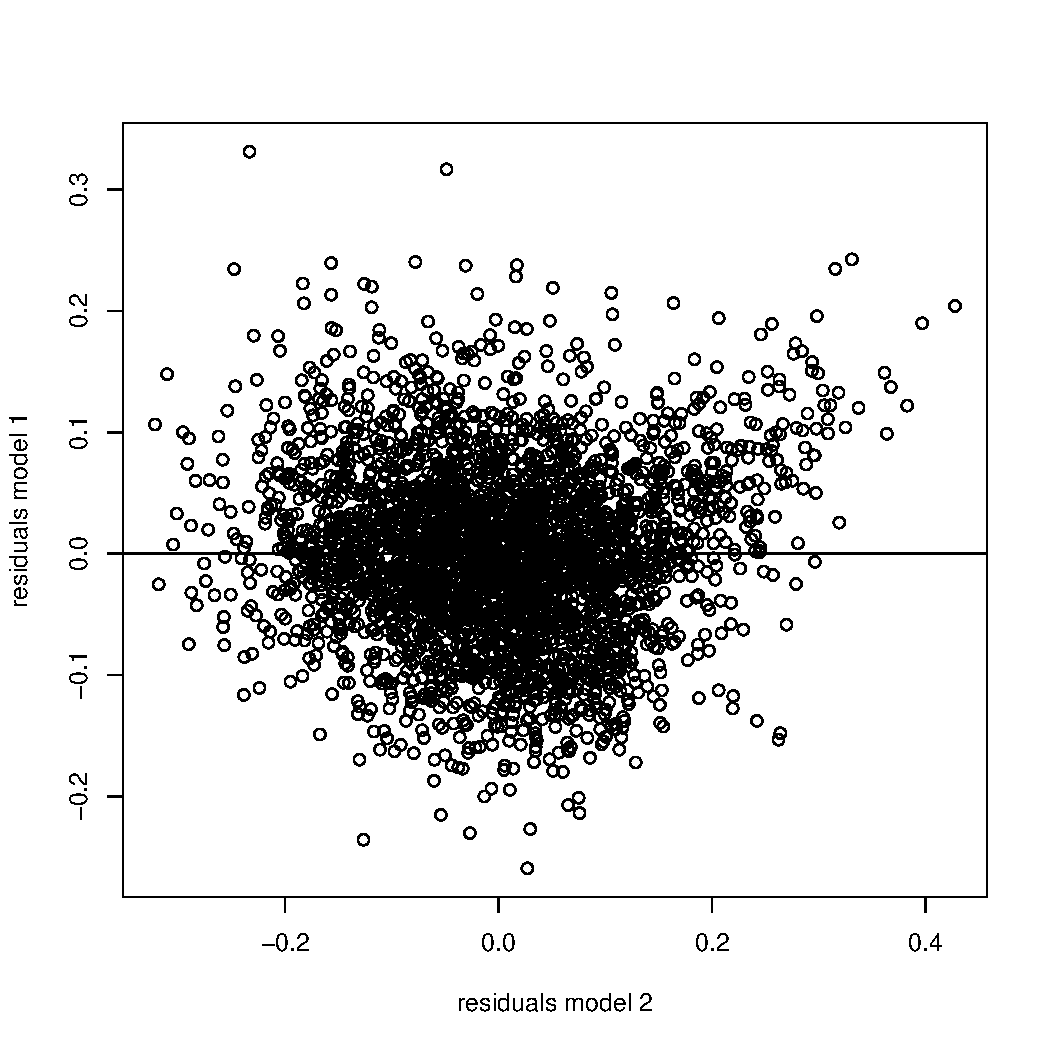
\includegraphics[width=.85\textwidth]{res4.pdf}
			\end{figure}		
			Fig. \ref{fig:res_4}shows residuals are randomly arranged around 0, which means that the linear regression is accurate here.
		\item Write the prediction equation.\\
			Considering $\hat{Y}$ the predictor of \texttt{ lm1\_residuals}, \\ $\hat{\beta_0}$ the calculated coefficient,\\ $\hat{\beta_1}$ the calculated intercept,\\ $X$ the
			 \texttt{lm2\_residuals} \\ and the margin of error $\epsilon \leadsto  \mathcal{N} ( \mu, \sigma ), ( \mu, \sigma ) \in \mathds{R}\times \mathds{R}^+$, \\
			 the linear regression model gives:
			
			\begin{align*}
				 \hat{Y} &= \hat{\beta_1} X + \hat{\beta_0} + \epsilon \\
				&=   0.2569  X -5.934*10^{-18}  + \epsilon
			\end{align*}
	\end{enumerate}
	
	\newpage	

\section*{Question 5}
\noindent What if the incumbent's vote share is affected by both the president's popularity and the difference in spending between incumbent and challenger? 
	\begin{enumerate}
		\item Run a regression where the outcome variable is the incumbent's \texttt{voteshare} and the explanatory variables are \texttt{difflog} and \texttt{presvote}. \\
		The linear regression is done by the folowing code:
			\lstinputlisting[language=R, firstline=117, lastline=117]{PS03_victor_gomez_24362159.R}  
			which gives:
			\begin{verbatim}
				> lm5

				Call:
				lm(formula = voteshare ~ difflog + presvote, data = df)
				
				Coefficients:
				(Intercept)      difflog     presvote  
				    0.44864      0.03554      0.25688  
			\end{verbatim}	
			The scatter plot is made by the folowing code:
			\lstinputlisting[language=R, firstline=121, lastline=126]{PS03_victor_gomez_24362159.R}  
			Which gives the Fig.\ref{fig:lm_5}. \\
				
			\begin{figure}[h!]\centering
				\caption{\footnotesize Regression between \texttt{voteshare} and  variables  \texttt{difflog} and \texttt{presvote}}
				\label{fig:lm_5}
				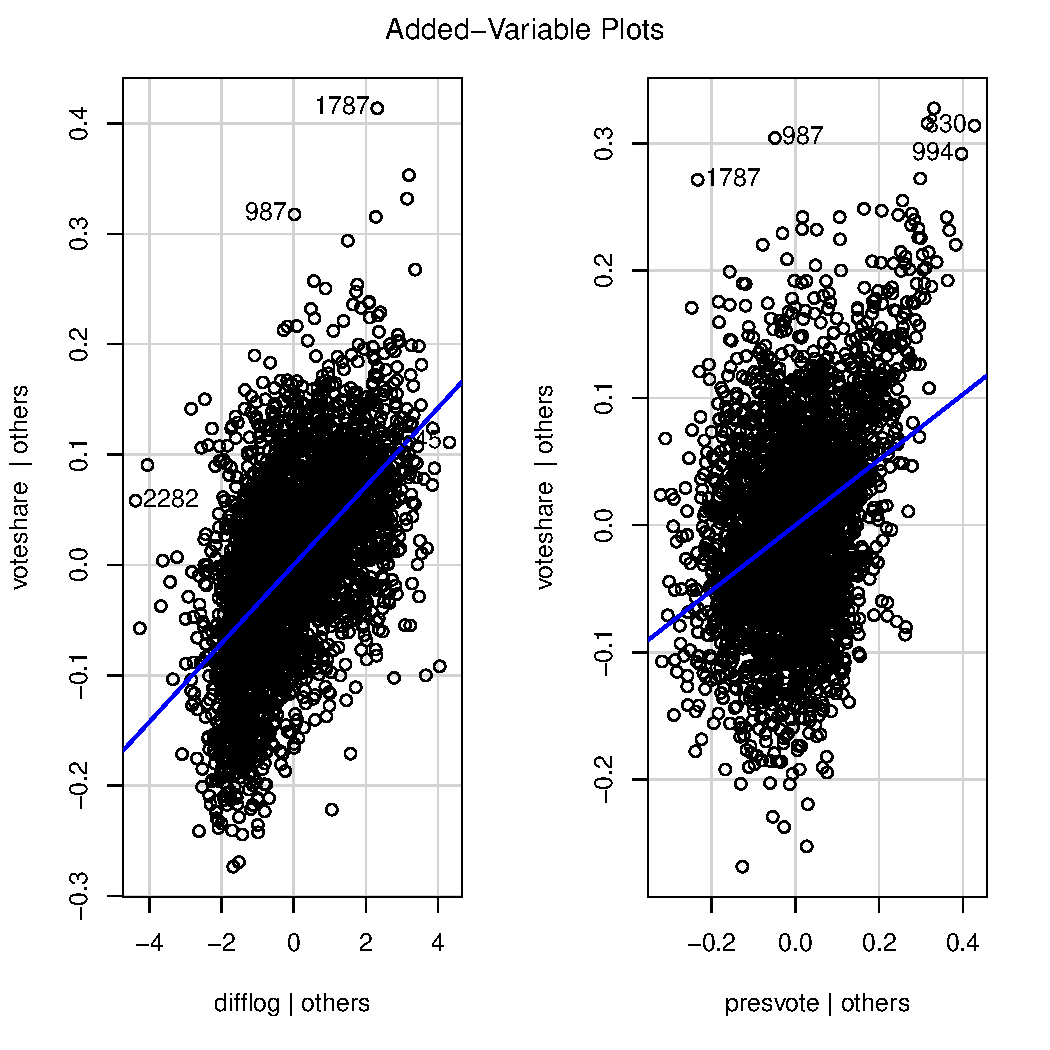
\includegraphics[width=.85\textwidth]{lm5.pdf}
			\end{figure}
			
		\item Write the prediction equation.	\\
		Considering $\hat{Y}$ the predictor of \texttt{voteshare}, \\ $\hat{\beta_2}$ the slope along \texttt{difflog} ,\\  $\hat{\beta_1}$ the slope along \texttt{presvote} ,\\
			 $\hat{\beta_0}$ the calculated intercept,\\ $X_2$ the  \texttt{difflog} \\ $X_1$ the  \texttt{presvote} \\
			 and the margin of error $\epsilon \leadsto  \mathcal{N} ( \mu, \sigma ), ( \mu, \sigma ) \in \mathds{R}\times \mathds{R}^+$, \\
			 the linear regression model gives:
			
			\begin{align*}
				 \hat{Y} &= \hat{\beta_2} X_2 + \hat{\beta_1} X_1 + \hat{\beta_0} + \epsilon \\
				&=    0.03554 X_2 + 0.25688   X_1 +  0.44864   + \epsilon
			\end{align*}
		\item What is it in this output that is identical to the output in Question 4? Why do you think this is the case?\\
			The slope of the model of Question 4 is the same is equal to the slope  $\hat{\beta_1}$ of this model.
			That would mean that the variability of \texttt{voteshare} not explained by  \texttt{difflog}  is due almost entirely to  \texttt{presvote}. Question 4 aimed to guess 			if there were a relationship between two unmodelised variations (in models of Questions 1 and 2).
	\end{enumerate}




\end{document}
